\documentclass[a4paper,14pt]{extreport} % формат документа

\usepackage{amsmath}
\usepackage{cmap} % поиск в ПДФ
\usepackage[T2A]{fontenc} % кодировка
\usepackage[utf8]{inputenc} % кодировка исходного текста
\usepackage[english,russian]{babel} % локализация и переносы
\usepackage[left = 2cm, right = 1cm, top = 2cm, bottom = 2 cm]{geometry} % поля
\usepackage{listings}
\usepackage{graphicx} % для вставки рисунков
\usepackage{amsmath}
\usepackage{float}
\usepackage{multirow}
\graphicspath{{images/}}
\DeclareGraphicsExtensions{.pdf,.png,.jpg}
\newcommand{\anonsection}[1]{\section*{#1}\addcontentsline{toc}{section}{#1}}

\lstset{ %
	language=C,                % Язык программирования 
	numbers=left,                   % С какой стороны нумеровать          
	frame=single,                    % Добавить рамку
	basicstyle=\small,
    escapebegin=\begin{russian}\commentfont,
    escapeend=\end{russian},
    literate={Ö}{{\"O}}1
    {Ä}{{\"A}}1
    {Ü}{{\"U}}1
    {ß}{{\ss}}1
    {ü}{{\"u}}1
    {ä}{{\"a}}1
    {ö}{{\"o}}1
    {~}{{\textasciitilde}}1
    {а}{{\selectfont\char224}}1
    {б}{{\selectfont\char225}}1
    {в}{{\selectfont\char226}}1
    {г}{{\selectfont\char227}}1
    {д}{{\selectfont\char228}}1
    {е}{{\selectfont\char229}}1
    {ё}{{\"e}}1
    {ж}{{\selectfont\char230}}1
    {з}{{\selectfont\char231}}1
    {и}{{\selectfont\char232}}1
    {й}{{\selectfont\char233}}1
    {к}{{\selectfont\char234}}1
    {л}{{\selectfont\char235}}1
    {м}{{\selectfont\char236}}1
    {н}{{\selectfont\char237}}1
    {о}{{\selectfont\char238}}1
    {п}{{\selectfont\char239}}1
    {р}{{\selectfont\char240}}1
    {с}{{\selectfont\char241}}1
    {т}{{\selectfont\char242}}1
    {у}{{\selectfont\char243}}1
    {ф}{{\selectfont\char244}}1
    {х}{{\selectfont\char245}}1
    {ц}{{\selectfont\char246}}1
    {ч}{{\selectfont\char247}}1
    {ш}{{\selectfont\char248}}1
    {щ}{{\selectfont\char249}}1
    {ъ}{{\selectfont\char250}}1
    {ы}{{\selectfont\char251}}1
    {ь}{{\selectfont\char252}}1
    {э}{{\selectfont\char253}}1
    {ю}{{\selectfont\char254}}1
    {я}{{\selectfont\char255}}1
    {А}{{\selectfont\char192}}1
    {Б}{{\selectfont\char193}}1
    {В}{{\selectfont\char194}}1
    {Г}{{\selectfont\char195}}1
    {Д}{{\selectfont\char196}}1
    {Е}{{\selectfont\char197}}1
    {Ё}{{\"E}}1
    {Ж}{{\selectfont\char198}}1
    {З}{{\selectfont\char199}}1
    {И}{{\selectfont\char200}}1
    {Й}{{\selectfont\char201}}1
    {К}{{\selectfont\char202}}1
    {Л}{{\selectfont\char203}}1
    {М}{{\selectfont\char204}}1
    {Н}{{\selectfont\char205}}1
    {О}{{\selectfont\char206}}1
    {П}{{\selectfont\char207}}1
    {Р}{{\selectfont\char208}}1
    {С}{{\selectfont\char209}}1
    {Т}{{\selectfont\char210}}1
    {У}{{\selectfont\char211}}1
    {Ф}{{\selectfont\char212}}1
    {Х}{{\selectfont\char213}}1
    {Ц}{{\selectfont\char214}}1
    {Ч}{{\selectfont\char215}}1
    {Ш}{{\selectfont\char216}}1
    {Щ}{{\selectfont\char217}}1
    {Ъ}{{\selectfont\char218}}1
    {Ы}{{\selectfont\char219}}1
    {Ь}{{\selectfont\char220}}1
    {Э}{{\selectfont\char221}}1
    {Ю}{{\selectfont\char222}}1
    {Я}{{\selectfont\char223}}1
    {і}{{\selectfont\char105}}1
    {ї}{{\selectfont\char168}}1
    {є}{{\selectfont\char185}}1
    {ґ}{{\selectfont\char160}}1
    {І}{{\selectfont\char73}}1
    {Ї}{{\selectfont\char136}}1
    {Є}{{\selectfont\char153}}1
    {Ґ}{{\selectfont\char128}}1
}

\begin{document}
\begin{titlepage}

    \begin{table}[H]
        \centering
        \footnotesize
        \begin{tabular}{cc}
            \multirow{8}{*}{
\includegraphics[scale=0.35]{bmstu}}
            & \\
            & \\
            & \textbf{Министерство науки и высшего образования Российской Федерации} \\
            & \textbf{Федеральное государственное бюджетное образовательное учреждение} \\
            & \textbf{высшего образования} \\
            & \textbf{<<Московский государственный технический} \\
            & \textbf{университет имени Н.Э. Баумана>>} \\
            & \textbf{(МГТУ им. Н.Э. Баумана)} \\
        \end{tabular}
    \end{table}

    \vspace{-2.5cm}

    \begin{flushleft}
        \rule[-1cm]{\textwidth}{3pt}
        \rule{\textwidth}{1pt}
    \end{flushleft}

    \begin{flushleft}
        \small
        ФАКУЛЬТЕТ
        \underline{<<Информатика и системы управления>>\ \ \ \ \ \ \ 
        \ \ \ \ \ \ \ \ \ \ \ \ \ \ \ \ \ \ \ \ \ \ \ \ \ \ \ \ \ \ \ 
    \ \ \ \ \ \ \ \ \ \ \ \ \ \ \ } \\
        КАФЕДРА
        \underline{<<Программное обеспечение ЭВМ и
        информационные технологии>>
        \ \ \ \ \ \ \ \ \ \ \ \ \ \ \ \ \ \ \ \ }
    \end{flushleft}

    \vspace{2cm}

    \begin{center}
        \textbf{Лабораторная работа № 8} \\
        \vspace{0.5cm}
    \end{center}

    \vspace{4cm}

    \begin{flushleft}
        \begin{tabular}{ll}
            \textbf{Дисциплина} & Операционные системы.  \\
            \textbf{Тема} & Создание виртуальной файловой системы.  \\
            \\
            \textbf{Студент} & Сиденко А.Г. \\
            \textbf{Группа} & ИУ7-63Б \\
            \textbf{Оценка (баллы)} & \\
            \textbf{Преподаватель} & Рязанова Н.Ю.   \\
        \end{tabular}
    \end{flushleft}

    \vspace{4cm}

   \begin{center}
        Москва, 2020 г.
    \end{center}

\end{titlepage}

\hfill

\textbf{md.c}

\begin{lstlisting}
#include <linux/init.h>
#include <linux/module.h>
#include <linux/kernel.h>
#include <linux/pagemap.h> 
#include <linux/fs.h> 
#include <asm/atomic.h>
#include <asm/uaccess.h>
#include <linux/slab.h>

MODULE_LICENSE("GPL");
MODULE_AUTHOR("Sidenko");
MODULE_DESCRIPTION("Lab8");

#define VFS_MAGIC_NUMBER 0x13131313
#define SLABNAME "vfs_cache"

// Размер элементов кэша
static int size = 7;
// Значение параметра из командной строки, иначе значение по умолчанию
module_param(size, int, 0);
static int number = 31;
// Значение параметра из командной строки, иначе значение по умолчанию
module_param(number, int, 0);

static void* *line = NULL;

// Конструктор вызывается при размещении каждого элемента
static void co(void* p)
{
  *(int*)p = (int)p;
}
struct kmem_cache *cache = NULL;

// Структура нужна для собственного inode
static struct vfs_inode
{
  int i_mode;
  unsigned long i_ino;
} vfs_inode;

// Создание inode
static struct inode * vfs_make_inode(struct super_block *sb, int mode)
{
  // Размещает новую структуру inode
  struct inode *ret = new_inode(sb);
  if (ret)
  {
    // mode определяет не только права доступа, но и тип
    inode_init_owner(ret, NULL, mode);
    // Заполнение значениями
    ret->i_size = PAGE_SIZE;
    ret->i_atime = ret->i_mtime = ret->i_ctime = current_time(ret);
    ret->i_private = &vfs_inode;
  }
  return ret;
}

// Печать строки, будет вызвана перед уничтожением суперблока
static void vfs_put_super(struct super_block *sb)
{
  printk(KERN_DEBUG "VFS super block destroyed!\n");
}

// Операции структуры суперблок
static struct super_operations const vfs_super_ops = {
	.put_super = vfs_put_super, // деструктор суперблока
	.statfs = simple_statfs,
	.drop_inode = generic_delete_inode,
};

// Функция инициализации суперблока
// Создание корневого каталога ФС
static int vfs_fill_sb(struct super_block *sb, void *data, int silent)
{
  struct inode* root = NULL;

  // Заполнение структуры
  sb->s_blocksize = PAGE_SIZE;
  sb->s_blocksize_bits = PAGE_SHIFT;
  sb->s_magic = VFS_MAGIC_NUMBER;
  sb->s_op = &vfs_super_ops;

  // Создание inode каталога ФС (указывает на это S_IFDIR)
  root = vfs_make_inode(sb, S_IFDIR | 0755);
  if (!root)
  {
    printk (KERN_ERR "VFS inode allocation failed !\n");
    return -ENOMEM;
  }

  // Файловые и inode-операции, которые мы назначаем новому inode
  root->i_op = &simple_dir_inode_operations;
  root->i_fop = &simple_dir_operations;

  // Создаем dentry для представления каталога в ядре
  sb->s_root = d_make_root(root);
  if (!sb->s_root)
  {
    printk(KERN_ERR "VFS root creation failed!\n");
    iput(root);
    return -ENOMEM;
  }
  return 0;
}

// Монтирование ФС
static struct dentry* vfs_mount(struct file_system_type *type, int flags, 
					const char *dev, void *data)
{
  // Так как виртуальная ФС, несвязанна с носителем, используем
  struct dentry* const entry=mount_nodev(type, flags, data, vfs_fill_sb);

  if (IS_ERR(entry))
    printk(KERN_ERR  "VFS mounting failed!\n");
  else
    printk(KERN_DEBUG "VFS mounted!\n");

  // Корневой каталог нашей ФС
  return entry;
}

// Описание создаваемой ФС
static struct file_system_type vfs_type  =  {
  .owner  =  THIS_MODULE, // счетчик ссылок на модуль
  .name  =  "vfs", // название ФС
  .mount  =  vfs_mount, // функция, вызываемая при монтировании ФС
  .kill_sb  =  kill_litter_super, // функция, вызываемая при 
  				  // размонтировании ФС
};

// Инициализация модуля
static int __init vfs_module_init(void)
{
  int i;

  if(size < 0)
  {
    printk(KERN_ERR "VFS_MODULE invalid sizeof objects\n");
    return -EINVAL;
  }

  // Выделение области, является непрерывной в физической памяти
  line = kmalloc(sizeof(void*) *number, GFP_KERNEL);
  if(!line)
  {
    printk(KERN_ERR "VFS_MODULE kmalloc error\n");
    kfree(line);
    return -ENOMEM;
  }

  // Инициализация области значениями
  for(i = 0; i < number; i++)
    line[i] = NULL;

  // Создание слаба
  // Расположение каждого элемента в слабе выравнивается по строкам
  cache = kmem_cache_create(SLABNAME, size, 0, SLAB_HWCACHE_ALIGN, co);

  if(!cache)
  {
    printk(KERN_ERR "VFS_MODULE cannot create cache\n");
    // Уничтожени слаба
    kmem_cache_destroy(cache);
    return -ENOMEM;
  }

  for(i = 0; i < number; i++)
  {
    // Выделение объектов
    if(NULL == (line[i] = kmem_cache_alloc(cache, GFP_KERNEL)))
    {
      printk(KERN_ERR "VFS_MODULE cannot alloc cache\n");
      for(i = 0; i < number; i++ )
        kmem_cache_free(cache, line[i]);
      return -ENOMEM;
    }
  }

  printk(KERN_INFO "VFS_MODULE allocate %d objects into slab: %s\n", 
  						number, SLABNAME);
  printk(KERN_INFO "VFS_MODULE object size %d bytes, full size %ld bytes\n",
  					 size, (long)size *number);

  // Регистрация файловой ситемы
  int ret = register_filesystem(&vfs_type);
  if (ret != 0)
  {
    printk(KERN_ERR "VFS_MODULE cannot register filesystem!\n");
    return ret;
  }

  printk(KERN_DEBUG "VFS_MODULE loaded!\n");
  return 0;
}

// Выход загружаемого модуля
static void __exit vfs_module_exit(void)
{
  int i;
  for(i = 0; i < number; i++)
  {
    // Возвращение объектов
    kmem_cache_free(cache, line[i]);
  }

  // Уничтожени слаба
  kmem_cache_destroy(cache);
  kfree(line);

  // Дерегистрация
  if (unregister_filesystem(&vfs_type) != 0)
  {
    printk(KERN_ERR "VFS_MODULE cannot unregister filesystem!\n");
  }

  printk(KERN_DEBUG "VFS_MODULE unloaded!\n");
}

module_init(vfs_module_init);
module_exit(vfs_module_exit);
\end{lstlisting}

\textbf{Makefile}

\begin{lstlisting}
ifneq ($(KERNELRELEASE),)
	obj-m := md.o
else
	CURRENT = $(shell uname -r)
	KDIR = /lib/modules/$(CURRENT)/build
	PWD = $(shell pwd)

default:
	$(MAKE) -C $(KDIR) M=$(PWD) modules

clean:
	rm -rf .tmp_versions
	rm *.ko
	rm *.o
	rm *.mod.c
	rm *.symvers
	rm *.order

endif
\end{lstlisting}

\begin{enumerate}
\item Загрузим модуль ядра и проверим в списке загруженных модулей ядра

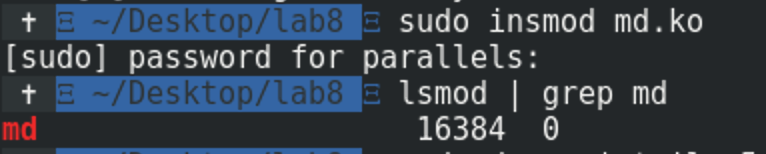
\includegraphics[scale=0.8]{1}

\item Вывод буфера сообщений ядра в стандартный поток вывода

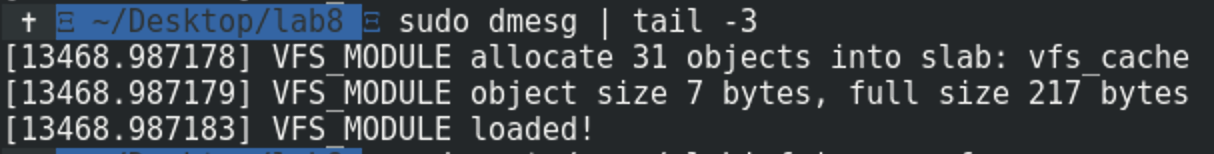
\includegraphics[scale=0.8]{2}

\item Посмотрим содержимое файла /proc/slabinfo, в котором хранится информация о кэшах

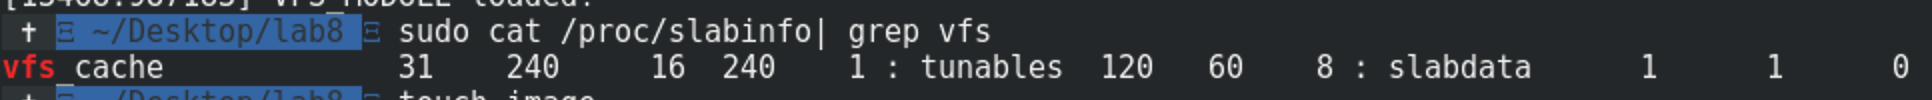
\includegraphics[scale=0.5]{3}

\item Создадим образ диска, пока он не хранит никаких данных. Создадим каталог, который будет точкой монтирования (корнем) файловой системы. Далее, используя этот образ, примонтируем файловую систему. 

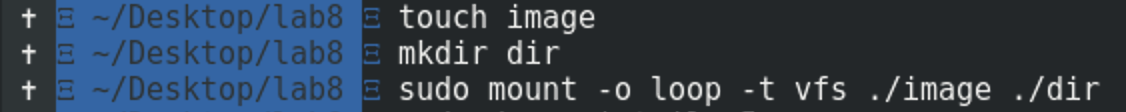
\includegraphics[scale=0.8]{4}

\item Вывод буфера сообщений ядра в стандартный поток вывода

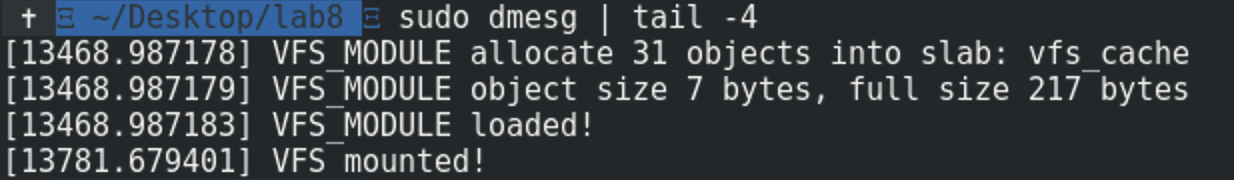
\includegraphics[scale=0.8]{5}

\item Размонтируем ФС и выгрузим модуль ядра. 

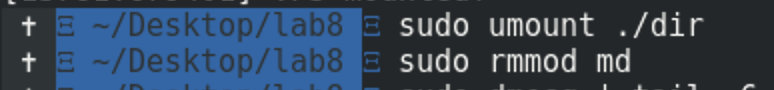
\includegraphics[scale=0.8]{6}

\item Вывод буфера сообщений ядра в стандартный поток вывода

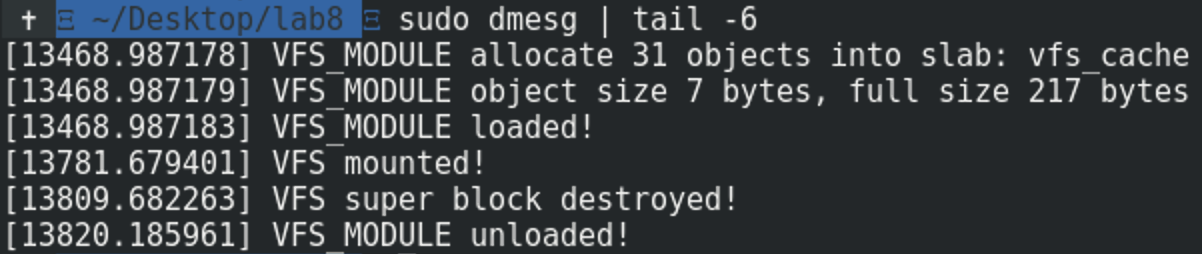
\includegraphics[scale=0.8]{7}

\item Также в программе предумотрено задание размера и количества элементов кэша

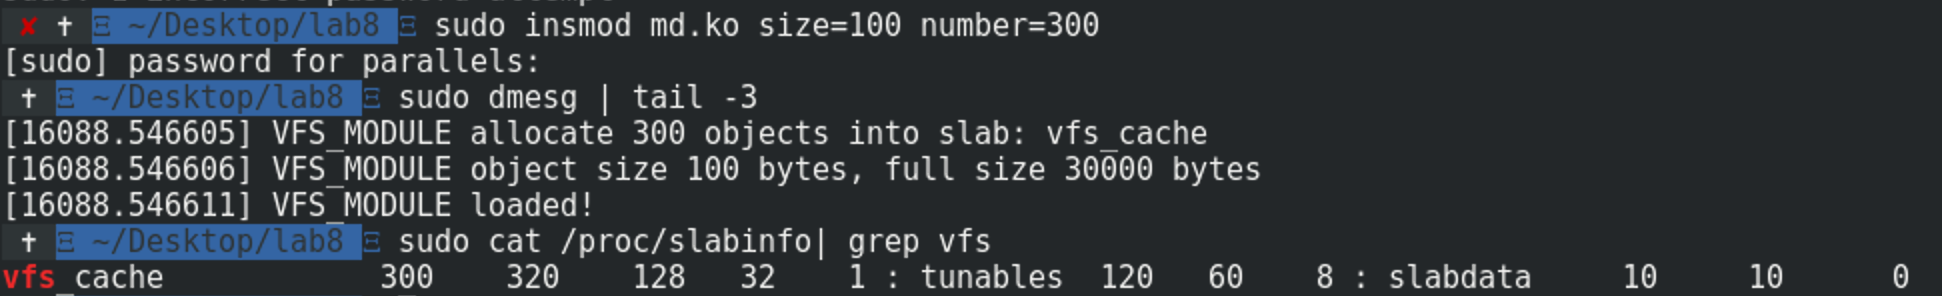
\includegraphics[scale=0.5]{8}

\end{enumerate}



\end{document}